\documentclass{beamer}

\usefonttheme{professionalfonts} % using non standard fonts for beamer
\usefonttheme{serif} % default family is serif

\usepackage{hyperref}
%\usepackage{minted}
\usepackage{animate}
\usepackage{graphicx}
\def\Put(#1,#2)#3{\leavevmode\makebox(0,0){\put(#1,#2){#3}}}
\usepackage{colortbl}
\usepackage{tikz}
\usepackage{amssymb}
\usepackage{enumerate}
\usepackage{arydshln}
\usepackage{algorithm}
\usepackage{algpseudocode}

\colorlet{lightred}{red!25}
\colorlet{lightgreen}{green!25}
\beamertemplatenavigationsymbolsempty

\newcommand\blfootnote[1]{%
  \begingroup
  \renewcommand\thefootnote{}\footnote{#1}%
  \addtocounter{footnote}{-1}%
  \endgroup
}

\makeatletter

%% Textclass specific LaTeX commands.
\newcommand\makebeamertitle{\frame{\maketitle}}%
\AtBeginDocument{%
  \let\origtableofcontents=\tableofcontents
  \def\tableofcontents{\@ifnextchar[{\origtableofcontents}{\gobbletableofcontents}}
  \def\gobbletableofcontents#1{\origtableofcontents}
}
%% User specified LaTeX commands.
\usetheme{Malmoe}
\useoutertheme{infolines}
\addtobeamertemplate{headline}{}{\vskip2pt}
\setbeamercovered{transparent}

\makeatother

%%%%%%%%%%%%%%%%%%%%%%%%%%%%%%%%%%%%%%
%% Main document
%%%%%%%%%%%%%%%%%%%%%%%%%%%%%%%%%%%%%%
\begin{document}
\title[PFLOCK report]{PFLOCK Report}
\author[AC]{Andres Calderon}
\institute[Spring'20]{University of California, Riverside}
\makebeamertitle
\newif\iflattersubsect

\AtBeginSection[] {
    \begin{frame}<beamer>
    \frametitle{Outline} 
    \tableofcontents[currentsection]  
    \end{frame}
    \lattersubsectfalse
}

\AtBeginSubsection[] {
    \begin{frame}<beamer>
    \frametitle{Outline} 
    \tableofcontents[currentsubsection]  
    \end{frame}
}

\begin{frame}{Point distribution per cell}
  \centering
  \begin{tabular}{c c c c c c}
  \hline
  Partitions  & Partitions     & avg    &                sd &                 min &   max \\
  requested & created       &           &                       &                       &           \\ 
  \hline
36 &         94 &          536.35 & 342.43 &  3 &     1524 \\
48 &        118 &         427.26 & 274.22 & 3 &     1208 \\
60 &         160 &         315.1 &  215.96 & 3 &     1057 \\
72 &         193 &         261.22 & 196.39 &  3 &     1057 \\
84 &         235 &         214.53 & 165.38 & 3 &     948  \\
96 &         274 &         184.0 & 130.47 & 3 &     842  \\
108 &        322 &         156.57 & 113.45 & 3 &     842 \\ 
120 &        322 &         156.57 & 113.45 & 3 &     842  \\
\hline
  \end{tabular}

\end{frame}

\begin{frame}{Duration per cell}
  \centering
  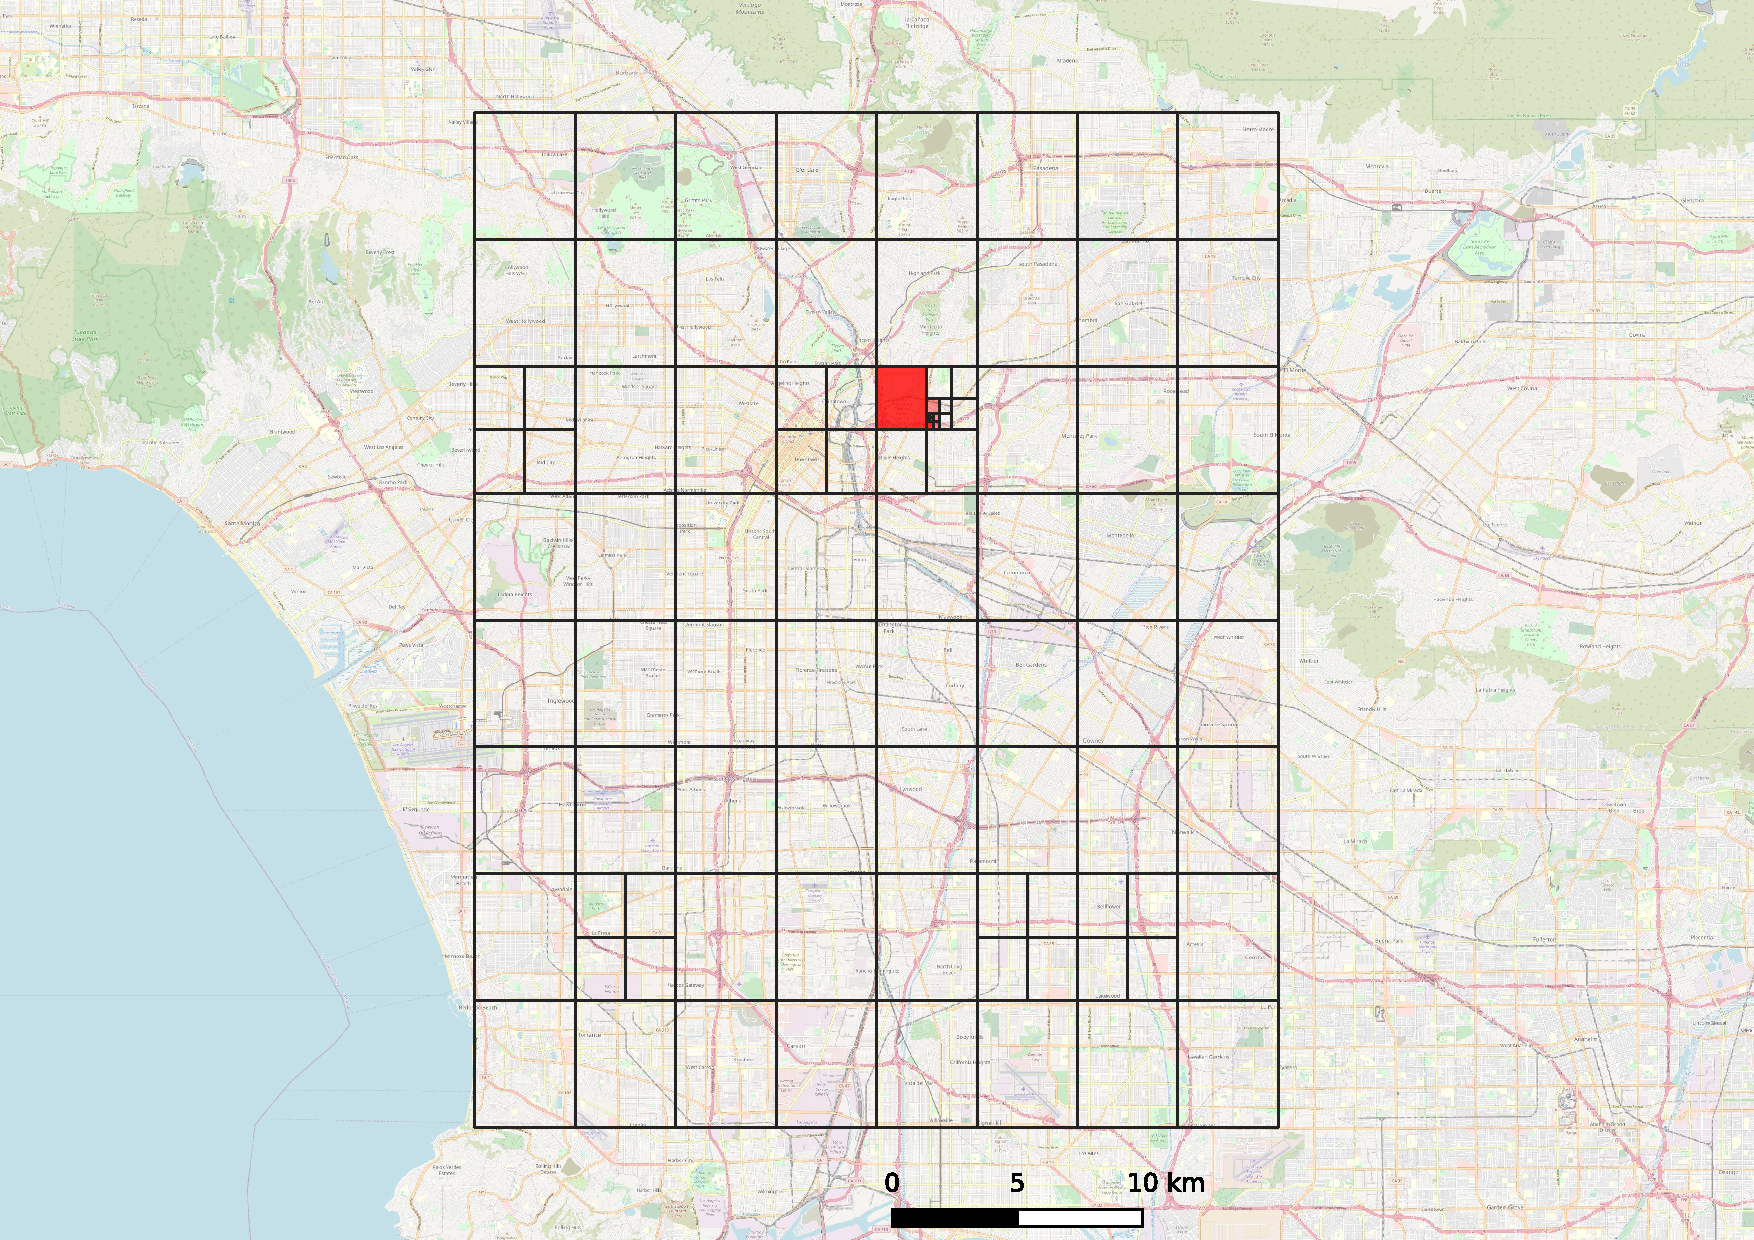
\includegraphics[width=0.9\textwidth]{figures/LA2}
\end{frame}

\begin{frame}{Point/Centers distribution per partition}{Partitions requested=36}
  \centering
    % latex table generated in R 3.6.1 by xtable 1.8-4 package
% Fri Aug 14 12:53:28 2020
\begin{table}[ht]
\centering
\resizebox{0.9\textwidth}{!}{%
\begin{tabular}{rrrrrrr}
  \hline
 & partitionId & pointsIn & pointsOut & centersIn & centeresOut & duration \\ 
  \hline
  1 & 38 & 454 & 300 & 10226 & 4728 & 28646.90 \\ 
  2 & 37 & 396 & 243 & 6261  & 3983 & 15458.30 \\ 
  3 & 40 & 254 & 157 & 4750  & 2844 & 14491.10 \\ 
  4 & 36 & 283 & 230 & 4522  & 3424 & 10504.60 \\ 
  5 & 30 & 416 & 83  & 4410  & 874  & 7630.10  \\ 
  6 & 39 & 199 & 185 & 2411  & 2857 & 3389.20  \\ 
  7 & 35 & 154 & 150 & 2663  & 2475 & 3184.50  \\ 
  8 & 33 & 100 & 60  & 595   & 959  & 1387.40  \\ 
  9 & 41 & 82  & 57  & 1402  & 894  & 1040.50  \\ 
   \hline
\end{tabular}%
}
\end{table}

\end{frame}
\begin{frame}{Point/Centers distribution per partition}
  \centering
  \includegraphics[width=0.9\textwidth]{figures/TP036}
\end{frame}

\begin{frame}{Point/Centers distribution per partition}{Partitions requested=108}
  \centering
    % latex table generated in R 3.6.1 by xtable 1.8-4 package
% Fri Aug 14 12:53:28 2020
\begin{table}[ht]
\centering
\resizebox{0.9\textwidth}{!}{%
\begin{tabular}{rrrrrrr}
  \hline
 & partitionId & pointsIn & pointsOut & centersIn & centeresOut & duration \\ 
  \hline
	1  & 142 & 254 & 157 & 4750 & 2844 & 14832.20 \\ 
	2  & 140 & 61  & 317 & 1781 & 6735 & 11930.00 \\ 
	3  & 139 & 162 & 164 & 4130 & 2694 & 8667.00  \\ 
	4  & 123 & 416 & 83  & 4410 & 874  & 7415.20  \\ 
	5  & 134 & 145 & 204 & 2955 & 3339 & 5532.50  \\ 
	6  & 137 & 141 & 209 & 2824 & 3948 & 5469.40  \\ 
	7  & 141 & 199 & 185 & 2411 & 2857 & 3271.50  \\ 
	8  & 135 & 96  & 151 & 1378 & 2216 & 3248.20  \\ 
	9  & 128 & 154 & 150 & 2663 & 2475 & 2998.60  \\ 
	10 & 138 & 90  & 136 & 1491 & 2847 & 2710.90  \\ 
	11 & 129 & 98  & 64  & 1743 & 951  & 2451.40  \\ 
	12 & 131 & 65  & 203 & 952  & 3440 & 2366.60  \\ 
	13 & 126 & 100 & 60  & 595  & 959  & 1535.50  \\ 
	14 & 133 & 112 & 71  & 1741 & 583  & 1446.60  \\ 
	15 & 132 & 68  & 58  & 1261 & 517  & 1134.20  \\ 
   \hline
\end{tabular}%
}
\end{table}

\end{frame}
\begin{frame}{Point/Centers distribution per partition}
  \centering
  \includegraphics[width=0.9\textwidth]{figures/TP108}
\end{frame}

\end{document}

